\section{Introduction}
L'arithmétique\footnote{Du grec ancien \guillemets{arithmos} qui signifie \guillemets{nombre}.} a pour objet l'étude des nombres entiers.
Ces entiers peuvent être naturels $(\mathbb{N}=\{0,1,2,3, \ldots\})$ ou relatifs $(\mathbb{Z}=\{\ldots,-3,-2,-1,0,1,2,3, \ldots\})$.

\smallskip

L'arithmétique est, avec la géométrie, une des plus anciennes branches des mathématiques et son origine remonte déjà à l'époque des égyptiens et des babyloniens, qui utilisaient des tables numériques pour calculer et résoudre des problèmes.
%\textgreek{'arijm'os}


\smallskip
Les intérêts de l'arithmétique sont multiples. Par exemple, considérons la situation suivante :
\begin{center}\begin{minipage}[t]{0.85\textwidth}\begin{center}
\textit{``Deux corps célestes $A$ et $B$ ont une fréquence d'apparition de respectivement 105 jours et 81 jours. Un astronome observe le corps $A$ le 27 décembre 2020 et le corps $B$ le 2 janvier 2021. Quelle est la prochaine date où les corps $A$ et $B$ apparaîtront simultanément?''}
\end{center}\end{minipage}\end{center}

Ce problème peut être modélisée à l'aide d'une équation \textit{diophantienne}, que nous apprendrons à résoudre et pourrons ainsi répondre à la question.

\smallskip
Un autre domaine d'importance de l'arithmétique est son application en \textit{cryptographie}. Comme nous le verrons tout au long de ces deux années, l'arithmétique joue un rôle essentiel dans le codage et le décodage de messages par différentes méthodes. La cryptographie RSA repose entièrement sur les concepts de l'arithmétique des \textit{nombres premiers}.
% la recherche de solutions \textbf{entières} d'une équation par exemple se révèle être très intéressante et, surtout, d'une grande utilité dans des domaines. En effet, la résolution d'équations dans l'ensemble des nombres relatifs 


\section{Division Euclidienne}
\subsection{Définition de la division euclidienne}

La division euclidienne, ou division avec reste, est nommée ainsi en hommage au mathématicien grec Euclide\footnote{Euclide d'Alexandrie était un mathématicien de la Grèce antique qui vécut aux environs de 300 av. JC. Son ouvrage \textit{Les Eléments}  est un des plus anciens et plus célèbres ouvrages des mathématiques.} qui  a été le premier (\textit{connu}) à formaliser et à prouver mathématiquement les propriétés fondamentales de cette opération dans son livre \textit{Les Éléments}.

\medskip
La division euclidienne, plus particulièrement l'algorithme permettent d'effectuer la dite division, est connue depuis l'école primaire. Cependant, à notre niveau il sera  nécessaire de présenter certains résultats de manière plus rigoureuse. Nous allons commencer par démontrer que le \\\guillemets{quotient} et le \guillemets{reste} de la division euclidienne existent toujours et sont uniques. C'est l'objet du théorème qui suit. %nous allons étudier


\begin{theoreme}[\normalsize\textit{théorème de la division euclidienne}]\label{thm:div_eucl}
Soit $n\in\Z$ et $d\in\N^{\ast}$.
Il \textbf{existe} des entiers $q\in\Z$ et $r\in\N$ tels que 
$$n=d\cdot q+r \hspace{3mm}\textrm{avec}\hspace{3mm} 0\leqslant r < d$$

De plus $q$ et $r$ \textbs{sont uniques}.
\end{theoreme}
\clearpage

\begin{demonstration}
~
%\centerline{\textit{\uline{Existence de $q$ et $r$}}}
\centerline{\textbsc{Existence de $\bm{q}$ et $\bm{r}$}}

\bigskip
Soient $n$ et $d$ des entiers comme dans l'hypothèse du théorème.

\smallskip
Pour simplifier et sans perte de généralité nous allons supposer que $n\geqslant 0$.

\bigskip
Considérons l'ensemble $S$ suivant :
$$S=\lbrace k\in \N \eh{2}\vert\eh{2} d\cdot k \leqslant n\rbrace$$

{Exemple : Pour $n=19$ et $d=3$ on a $S=\lbrace 0; 1; 2; 3; 4; 5; 6\rbrace$ }

\medskip
L'ensemble $S$ vérifie les 3 conditions suivantes :
\begin{enumerate}[label=\textbf{\roman*)}]
\item $S$ est non-vide car $0\in S$.
\item $S$ est un ensemble majoré car pour $k\in S$ on a $k\leqslant n$.\\
(l'ensemble est majoré par $n$).
\item C'est un ensemble fini car il ne contient que des nombres entiers positifs inférieurs à $n$.
\end{enumerate}

Donc $S$ possède un plus grand élément qu'on note $q=max(S)$.

\medskip

De plus on a : \hspace{2mm}\begin{minipage}[t]{0.8\textwidth}$d q \leqslant n$ \eh{1}(car $q\in S$) \et{1} $d (q+1)>n$ \eh{1}(car $(q+1)\notin S$).\end{minipage}

\smallskip
Donc : $$d q \leqslant n \leqslant d (q+1)$$
$$\ssi[2]d q \leqslant n \leqslant d q+d $$
$$\ssi[2]0\leqslant \underbrace{n-dq}_{=r}<d$$

Finalement nous obtenons : 
$$n=\overbrace{d q+\underbrace{(n-dq)}_{=r}}^{=n}\eh{4}\textrm{avec }\eh{2} 0\leqslant n-dq<d$$

Et donc :
$$n=d q+r\eh{4}\textrm{avec }\eh{2} 0\leqslant r<d$$


\vspace{2mm}
\centerline{\textbsc{Unicité de $\bm{q}$ et $\bm{r}$}}

\bigskip\renewcommand{\arraystretch}{1.2}
Supposons que : \hspace{2mm}$\left\lbrace\begin{tabular}{@{\hspace{1mm}}l}
$n=d q_1+r_1 \hspace{3mm}\textrm{avec}\hspace{3mm} 0\leqslant r_1 < d$\\
$n=d q_2+r_2 \hspace{3mm}\textrm{avec}\hspace{3mm} 0\leqslant r_2 < d$
\end{tabular}\right.$. \eh{1}Donc on a : 
$$d q_1+r_1=d q_2+r_2 \eh{2}(E)$$

%$$d\cdot q_1+r_1=d\cdot q_2+r_2\tag{R \theequation}$$

\smallskip
Si on avait $q_2>q_1$ (donc $q_2\geqslant q_1+1$) on aurait :
$$r_1=d q_2-d q_1+r_2$$
$$r_1=d\underbrace{(q_2-q_1)}_{\geqslant 1}+\underbrace{r_2}_{\geqslant 0}\geqslant d $$

\smallskip
Ce qui est une contradiction puisque $r_1<d$.

\smallskip
On fait le même raisonnement en supposant que $q_1>q_2$ et on arrive à la même contradiction.

\medskip
Finalement, on conclut que nécessairement $q_1=q_2$ et par suite, en remplaçant dans l'égalité (E), on a trouve également que $r_1=r_2$.

\hfill $\blacksquare$
\end{demonstration}

\begin{exemples}{1mm}
	\item  La division euclidienne de $114$ par $8$ correspond à : $114 = 8 \cdot 14 + 2$.
	
	Ainsi $q = 14$ et $r = 2$.
	
	\vspace{0.3cm}
	
	\item Pour avoir un reste positif dans la division euclidienne de $-114$ par $8$, on écrit : $-2 = 6 - 8$.
	
	On obtient alors : $-114 = 8 \cdot (-14) - 2 = 8 \cdot (-14) - 8 + 6 = 8 \cdot (-15) + 6$.
	
	Ainsi $q = -15$ et $r = 6$.
\end{exemples}

\medskip
\begin{definition}
\textbf{Diviser} un nombre relatif $n$ par un nombre naturel $d$ c'est déterminer les nombres $q$ et $r$ comme dans le théorème \ref*{thm:div_eucl}.

\medskip
On appelle $q$ est le \textbs{quotient} de la division et $r$ est le \textbs{reste} de la division. 
\end{definition}




\begin{definition}
Soient $d\in \Z^{\ast}$ et $n\in \Z$.

\smallskip
On dit indistinctement que \guillemets{\textbs{$\bm d$ divise $\bm n$}} ou \guillemets{\textbs{$\bm d$ est un diviseur de $\bm n$}} ou \guillemets{\textbs{$\bm n$ est divisible par $\bm d$}} ou \guillemets{\textbs{$\bm n$ est un multiple de $\bm d$}}, s'il existe $q\in\Z$ tel que $n=q\cdot d$.

\medskip
Notation : \begin{minipage}[t]{0.8\textwidth}
Si $d$ divise $n$ on note $d\mid n$

\smallskip
Si $d$ ne divise pas $n$ on note $d\nmid n$
\end{minipage}
\end{definition}



\begin{exemples}{0mm}
\item $5\mid 20\;$ car $\;20=5\cdot \underbrace{4}_{=q}$
\item $-2\mid 6\;$ car $\;6=(-2)\cdot \underbrace{(-3)}_{=q}$

\end{exemples}




%\subsection{Propriétés de la division euclidienne}
\begin{proposition}[\normalsize\textit{propriétés de la division euclidienne}]
Soient $a$, $b$ et $c$ des nombres entiers non-nuls. Alors :
\begin{enumerate}[label=\roman*)]
\item $a\mid a$ pour tout $a\in \Z$.
\item Si $a\mid b$ et $b\neq 0\;$ alors $|a|\leqslant |b|$.
\item Si $a\mid b$ et $b\mid a\;$ alors $|a|= |b|$.
\item Si $a\mid b$ et $b\mid c\;$ alors $a\mid c$.
\item Si $a\mid b$ et $a\mid c\;$ alors $a\mid (xb+yc) \eh{2}$ quel que soit $\eh{1} x\; ;\;y \,\in\, \Z$.
\\ {\footnotesize ($a$ divise toute combinaison linéaire de $b$ et $c$)}
\end{enumerate}
\end{proposition}

\medskip
\noindent{\it Démonstration:}

\vspace{-2mm}
\begin{enumerate}[label=\roman*),itemsep=4mm]
\item Pour tout $a\in \Z$, il existe $q=1\,(\in \Z)$ tel que $a=a\cdot 1$. Donc  $a\mid a$ pour tout $a\in\Z$ . 
\item Comme $a\mid b$, alors il existe $q\in\Z$ tel que $b=aq$. Donc $|b|=|a|\cdot |q|$.

Comme $b\neq 0$ alors $a\neq 0$ et $q\neq 0$, donc nécessairement $|q|\geqslant 1$. On déduit alors que $|a|\leqslant|b|$.
\item On a : \renewcommand{\arraystretch}{1.5}
$\left\lbrace\begin{array}{l}
a\mid b \overset{\scriptscriptstyle{prop. ii)}}{\Rightarrow} |a|\leqslant |b|\\
b\mid a \overset{\scriptscriptstyle{prop. ii)}}{\Rightarrow} |b|\leqslant |a|
\end{array}\right\rbrace$ donc on en déduit que $|a|= |b|$.
\item Par définition on a : \renewcommand{\arraystretch}{1.5}
$\left\lbrace\begin{array}{l}
a\mid b \Rightarrow \textrm{ il existe } q\in\Z\textrm{ tel que } b=aq\\
b\mid c \Rightarrow \textrm{ il existe } q\in\Z\textrm{ tel que } c=bq'
\end{array}\right.$

Donc : $c=b\cdot q'=\underbrace{(a\cdot q)}_{=b}\cdot q'=a\cdot \underbrace{(q\cdot q')}_{=q''\in Z}=a\cdot q''$.

\smallskip
On conclut qu'il existe $q''\in Z$ tel que $c=a\cdot q''$. Par définition, cela signifie que $a\mid c$. 
\item Par définition on a : \renewcommand{\arraystretch}{1.5}
$\left\lbrace\begin{array}{l}
a\mid b \Rightarrow b=a\cdot q\in \Z\\
a\mid c \Rightarrow c=a\cdot q'\in \Z
\end{array}\right\rbrace$ alors pour tout $x, y \in \Z$ on a :
$$x\cdot b+y\cdot c=x\cdot\underbrace{(a\cdot q)}_{=b}+y\cdot\underbrace{(a\cdot q')}_{=c}=a\cdot\underbrace{(x\cdot q+y\cdot q')}_{=q''\in Z}=a\cdot q''$$

\smallskip
On conclut qu'il existe $q''\in Z$ tel que $xb+yc=a\cdot q''$

\smallskip
Par définition cela veut dire que $a\mid (xb+yc)$.

\hfill $\blacksquare$
\end{enumerate}

\medskip

\begin{remarque}
	Lorsque l'on  cherche à résoudre des problèmes en arithmétique, on peut traduire la situations en équations, mais pour la résolution en essayera de faire apparaître des expressions faisant intervenir des produits de nombres entiers comme dans l'exemple suivant.
\end{remarque}

\medskip

\begin{exemple}
	On veut résoudre le problème suivant:
	
	\begin{quote}
		Lorsqu'on divise $a$ par $b$, le reste est 8 et lorsqu'on divise $2a$ par $b$, le reste est 5. Déterminer le diviseur $b$.
	\end{quote} 
	
	
	Écrivons chacune des deux divisions euclidiennes, en notant $q$ et $q'$ les quotients respectifs :
	
	$$\begin{cases} a = b \cdot q + 8 \quad \text{avec} \quad b > 8 \\ 2a = b \cdot q' + 5 \quad \text{avec} \quad b > 5 \end{cases}$$
	
	En multipliant la première division par 2 et en égalisant avec la deuxième, on obtient :
	
	$$2b \cdot q + 16 = b \cdot q' + 5 \quad \text{avec} \quad b > 8$$
	
	$$b \cdot (2q - q') = -11$$
	
	$$b \cdot (q' - 2q) = 11$$
	
	$b$ est donc un multiple positif non nul de 11, supérieur à 8, donc l'unique possibilité est $b = 11$.
\end{exemple}

\begin{exstheorie}
\renewcommand{\eexo}{\vspace{4mm}}
\exo
Sans calculatrice, effectuer la division euclidienne de \nombre{91239123} par \nombre{8924}.


\eexo
\pagebreak[3]



\exo
Déterminer le quotient et le reste de la division euclidienne de $-17$ par $3$.


\eexo
\pagebreak[3]

\exo

\vspace{-0.8cm}
\begin{enumerate}
	\item[\textbf{a)}] Écrire la division euclidienne de : 
	\begin{enumerate}
		\item[\textbf{1)}] $23$ par $4$.
		\item[\textbf{2)}] $-23$ par $4$.
	\end{enumerate}
	
	\item[\textbf{b)}] La différence entre deux entiers naturels est $538$. Si l'on divise l'un par l'autre le quotient est $13$ et le reste $34$. Quels sont ces deux entiers naturels ?
	
	\item[\textbf{c)}] Déterminer un entier naturel $n$ qui, divisé par $23$ donne pour reste $1$ et, divisé par $17$ donne le même quotient et pour reste $13$.
	
	\item[\textbf{d)}] Le quotient d'un entier naturel $x$ par $3$ est $7$. Quels sont les restes possibles ? \\
	En déduire quelles sont les valeurs de $x$ possibles.
\end{enumerate}

\eexo
\pagebreak[3]


\exo
L'aiguille des secondes d'une montre indique 17 secondes. Combien de secondes indiquera-t-elle dans :
\begin{enumerate}[label=\alph*),itemsep=0mm,left=0mm]
\item 55 secondes.
\item 555 secondes.
\item 5555 secondes.
\end{enumerate}



\eexo
\pagebreak[3]



\exo
%Sachant que $96842=256 \cdot 375+842$, déterminer, sans effectuer la division, le reste de la division de 96842 par :
%\begin{enumerate}[label=\alph*)]
%\item 256
%\item 375
%\end{enumerate}
Le quotient d'un nombre entier naturel $n$ par 3 est 7. Quels sont les restes possibles?\\
En déduire les valeurs possibles pour $n$.




\eexo
\pagebreak[3]





\exo
Si on divise un nombre entier $a$ par 18, le reste est 13. Quelle est le reste de la division de $a$ par 6?





\eexo
\pagebreak[3]





\exo
Monter que $\forall\; n\in \N$ on a :
\begin{enumerate}[label=\alph*),left=0mm]
\item $n(n+1)(n+2)(n+3)$ est divisible par 24.
\item $n(n+1)(n+2)(n+3)(n+4)$ est divisible par 120.
\end{enumerate}






\eexo
\pagebreak[3]





\exo
Déterminer tous les entiers $a$ qui, divisés par $5$, donnent un quotient égal à 3 fois le reste.





\eexo
\pagebreak[3]





\exo
Sachant que $\nombre{96842}=256 \cdot 375+842$, déterminer, sans effectuer la division, le reste de la division de \nombre{96842} par :
%\leavevmode\vspace{-\dimexpr\baselineskip+\topsep}% Solution pour alignement trouvée sur https://tex.stackexchange.com/questions/456914/item-number-not-aligned-with-tasks

\medskip
\begin{tasks}[after-item-skip=2mm,before-skip=0mm,debug=false](2)%[before-skip=0mm,after-item-skip=-1mm,debug=false](2)
\task 256
\task 375
\end{tasks}




\eexo
\pagebreak[3]





\exo
\leavevmode\vspace{-\dimexpr\baselineskip+\topsep-2mm}% Solution pour alignement trouvée sur https://tex.stackexchange.com/questions/456914/item-number-not-aligned-with-tasks
\begin{tasks}[after-item-skip=2mm,before-skip=0mm,debug=false]%[before-skip=0mm,after-item-skip=-1mm,debug=false](2)
\task Montrer que la division euclidienne par 8 du carré de tout nombre naturel impair donne un reste de 1.
\task Montrer que la division euclidienne par 8 du carré de tout nombre naturel pair donne un reste de 0 ou de 4.
\end{tasks}

\vspace{-2mm}
\indication{1}{comment écrit-on un nombre pair? un nombre impair?}

%{\footnotesize \textsl{(\textbs{Indications :} comment écrit-on un nombre pair? un nombre impair?)}}





\eexo
\pagebreak[3]





\exo
Sans utiliser d'identités remarquables ou la formule du discriminant, déterminer tous les nombres relatifs qui sont solution de :

\medskip
\begin{tasks}[after-item-skip=2mm,before-skip=0mm,debug=false](2)%[before-skip=0mm,after-item-skip=-1mm,debug=false](2)
\task $n^2+n=20$
\task $n^2+2n=35$
\end{tasks}
%\begin{enumerate}[label=\alph*)]
%\item $n^2+n=20$
%\item $n^2+2n=35$
%\end{enumerate}
{\footnotesize \textsl{(\textbs{Indications :} faire une mise en évidence appropriée.)}}






\eexo
\pagebreak[3]





\exo
Résoudre dans $\N$ l'équation suivante :
$$x^2-2xy=15$$

\vspace{-2mm}
{\footnotesize \textsl{(\textbs{Indications :} factoriser à gauche.)}} 




\eexo





\exo
Soit $n$ un nombre naturel.

\vspace*{-2mm}
\begin{enumerate}[label=\roman*),itemsep=0mm,left=-1mm]
\item Montrer que $(n+1)^3=n^2(n+3)+3n+1$.
\item Déterminer l'ensemble des nombres entiers naturels tels que le reste de la division de $(n+1)^3$ par $n^2$ soit de $3n+1$.
\end{enumerate}


%\eexo
%\pagebreak[3]
%
%
%
%
%
%\exo
%A l'aide de la décomposition en nombre premiers, déterminer le pgdc des nombres suivants :
%\begin{enumerate}[label=\alph*)]
%\item 126 ; 230.
%\item 390 ; 720 ; 450.
%\item 180 ; 606 ; 750.
%\end{enumerate}
\end{exstheorie}

\clearpage


\subsection{PGDC et Algorithme d'Euclide}
\begin{definition}
Soient $a, b\in \Z$ non tous les deux nuls.\\
Le \textbs{plus grand diviseur commun} de $a$ et de $b$ est le plus grand entier positif qui divise à la fois $a$ et $b$. On le note $\pgdc(a;b)$
\end{definition}


\begin{proposition}\label{prop:pgdc_euclide}
Soient $n \in \Z$, $d\in \N^{\ast}$ et $q$ et $r$ respectivement le quotient et le reste de la division euclidienne de $n$ par $d$. Alors :
$$\pgdc(n;d)=\pgdc(d;r)$$
\end{proposition}


\begin{demonstration}
Nous allons démontrer que les diviseurs communs de $n$ et $d$ sont les mêmes que les diviseurs communs de $d$ et $r$.

\smallskip
Soit $a$ un diviseur de $d$ et de $n$ ($a\mid d$ et $a\mid n$). Par définition $a\mid d$, il faut montrer que $a\mid r$. 

Comme $a\mid d$ alors $a\mid q\cdot d$. De plus on sait que $a\mid n$. Donc :
$$a\mid \underbrace{n-q\cdot d}_{\textrm{\footnotesize comb. liné.}}=r \textrm{\eh{3}et donc \eh{3}} a\mid r$$

\smallskip 
Soit $b$ un diviseur de $d$ et de $r$ ($b\mid d$ et $b\mid r$). Par définition $b\mid d$, il faut montrer que $b\mid n$. 

Comme $b\mid d$ alors $b\mid q\cdot d$. De plus on sait que $b\mid r$. Donc :
$$b\mid \underbrace{q\cdot d+r}_{\textrm{\footnotesize comb. liné.}}=n \textrm{\eh{3}et donc \eh{3}} \Rightarrow b\mid n$$


On conclut que les diviseurs du couple $(n;d)$ sont les mêmes que ceux du couple $(d;r)$ et vice-versa. En particulier, le plus grand diviseur commun du couple $(n,d)$ doit être le même que celui de $(d,r)$.

\vspace{-1mm}\hfill $\blacksquare$
\end{demonstration}


\vspace{4mm}
\centerline{\textsc{Algorithme d'Euclide pour déterminer le $\pgdc(a;b)$}}

\medskip
On souhaite calculer le $\pgdc$ de $a, b\in \N^{\ast}$. On suppose $a\geqslant b$.

\smallskip
L'algorithme d'Euclide consiste à faire des divisions euclidiennes successives.
Le dernier reste non-nul est le $\pgdc$ cherché.

\vspace{-1mm}
\begin{itemize}
\item On divise $a$ par $b$ : $a=q_1\cdot b+r_1$ avec $0\leqslant r_1< b$.
	
On a $\pgdc(a;b)=\pgdc(b;r_1)$ {\footnotesize\textsl{(proposition \ref{prop:pgdc_euclide})}}

Si $r_1=0$ alors $\pgdc(a;b)=b$. Si $r_1\neq 0$ alors on continue.

\item On divise $b$ par $r_1$ : $b=q_2\cdot r_1+r_2$ avec $0\leqslant r_2< r_1$.
	
	On a $\pgdc(b;r_1)=\pgdc(r_1;r_2)$ {\footnotesize\textsl{(proposition \ref{prop:pgdc_euclide})}}
	
Si $r_2=0$ alors $\pgdc(b;r_1)=r_1$. Si $r_2\neq 0$ alors on continue.

%\item On divise $r_1$ par $r_2$ : $r_1=q_3\cdot r_2+r_3$ avec $0\leqslant r_3< r_2$
%	
%	On a $\pgdc(r_1;r_2)=\pgdc(r_2;r_3)$ {\footnotesize\textsl{(proposition \ref{prop:pgdc_euclide})}}
%	
%	Si $r_3=0$ alors $\pgdc(r_1;r_2)=r_2$
%	
%	Si $r_3\neq 0$ alors on continue.

\item $...$

\newcommand{\insertun}{\begin{minipage}{0.1\textwidth}
\centering\tiny dernier

reste non-nul

\vspace{1mm}
\end{minipage}}


%\item On divise $r_{k-2}$ par $r_{k-1}$ : $r_{k-2}=q_k\cdot r_{k-1}\overset{\textrm{\insertun}}{+\boxed{r_k}}$ avec $0\leqslant r_k< r_{k-1}$
%	
%	On a $\pgdc(r_{k-2};r_{k-1})=\pgdc(r_{k-1};r_k)$ {\footnotesize\textsl{(proposition \ref{prop:pgdc_euclide})}}
%	
%	%Si $r_3=0$ alors $pgdc(r_{k-2};r_{k-1})=r_{k-1}$
%	%
%	%Si $r_3\neq 0$ alors on continue.

\item On divise $r_{k-1}$ par $r_k$ : $r_{k-1}=q_{k+1}\cdot r_k+0$ 
	
	On a $\pgdc(r_{k-1};r_k)=r_k$ 
	
	%Si $r_3=0$ alors $pgdc(r_{k-2};r_{k-1})=r_{k-1}$
	%
	%Si $r_3\neq 0$ alors on continue.
\end{itemize} 

On conclut en remarquant que $\pgdc(a;b)=\pgdc(r_{k-1};r_k)=r_k$.

\medskip	
En appliquant cette algorithme, nous obtenons nécessairement un reste de $0$ en un nombre fini d'étapes.\\
En effet, nous engendrons une suite strictement décroissante de \guillemets{restes} tous entiers et positifs. Par ailleurs, il est possible de continuer l'algorithme tant que le reste ne vaut pas $0$. Nous arriverons donc obligatoirement à un reste de $0$ à une certaine étape.


\smallskip
\begin{exemple}
Calculons le $\pgdc(600;124)$ :

\vspace{-8mm}
\begin{center}
\psset{yunit=1cm,xunit=1cm,gridcolor=cgrille}
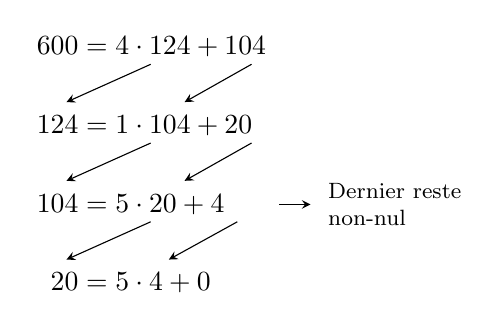
\begin{tikzpicture}[x=1cm, y=1cm, >=stealth]
	% Lignes d'équations
	\node[anchor=west] at (0, 3.5) {$600=4\cdot \boxed{124}+\boxed{104}$};
	\draw[->] (1.57, 3.28) -- (0.5, 2.8);
	\draw[->] (2.85, 3.28) -- (2, 2.8);
	
	\node[anchor=west] at (0, 2.5) {$124=1\cdot \boxed{104}+\boxed{20}$};
	\draw[->] (1.57, 2.28) -- (0.5, 1.8);
	\draw[->] (2.85, 2.28) -- (2, 1.8);
	
	\node[anchor=west] at (0, 1.5) {$104=5\cdot \boxed{20}+\boxed{4}$};
	\draw[->] (1.57, 1.28) -- (0.5, 0.8);
	\draw[->] (2.67, 1.28) -- (1.8, 0.8);
	
	\node[anchor=west] at (0, 0.5) {$\phantom{1}20=5\cdot 4+0$};
	
	% Flèche et annotation à droite
	\draw[->] (3.2, 1.5) -- (3.6, 1.5);
	\node[anchor=west, align=left, font=\footnotesize] at (3.7, 1.5) {Dernier reste\\ non-nul};
\end{tikzpicture}
\end{center}

On conclut que $\pgdc(600;124)=4$.
\end{exemple} 





%\vspace{6mm}
%
%\begin{enumerate}[label=\roman*)]
%\item A l'aide de l'algorithme d'Euclide, déterminer $\pgdc(9945;3003)$.
%\item Déterminer les couples d'entiers naturels de pgdc 18 et dont la somme vaut 360.
%\end{enumerate}




\begin{definition}
Soient $a; b \in \Z$. On dit que $a$ et $b$ sont \textbs{premiers entre eux} si \textbf{pgdc}$\bm{(a;b)=1}$.
\end{definition}




\begin{exemples}{3mm}
\item $\pgdc(18;25)=1$ car $\textrm{Div}_{18}=\{1;2;3;6;9;18\}$ \et{1} $\textrm{Div}_{25}=\{1;5;25\}$ \et{0.5} le plus grand diviseur commun entre les deux nombres est $1$.
\item Soit $a\in \Z$, alors $a$ et $a+1$ sont premiers entre eux.

En effet, soit $d$ un diviseur commun de $a$ et de $a+1$. (i.e. $d\mid a$ et $d\mid(a+1)$)

Donc $d\mid \underbrace{\big((a+1)-a\big)}_{\textrm{\footnotesize comb. liné.}}=1 \implique[2] d\mid 1$.


%\underbrace{n-q\cdot d}_{\textrm{\footnotesize comb. liné.}}
Par conséquent $d=-1$ ou $d=1$. On conclut que $\pgdc(a;a+1)=1$ et  donc $a$ et $(a+1)$ sont premiers entre eux.
\item Soient $a,b \in \Z$ \et{1} $d=\pgdc(a;b)$. La décomposition suivante peut être utile :

\vspace{-2mm}
$$
\left\lbrace\begin{array}{l}
a=a'\cdot d\\
b=b'\cdot d
\end{array}\right. \textrm{avec $a',b'\in \Z$ \et{2} $\pgdc(a';b')=1$}
$$
\end{exemples}


\vspace{1mm}


\begin{exstheorie}
\exo
Soit $a$ et $b$ $\in\N$ et tels que $\pgdc(a;b)=12$.

\smallskip
Les quotients successifs obtenus par l'algorithme d'Euclide sont : 8, 2 et 7.

\smallskip
Déterminer $a$ et $b$.


\medskip


\exo
A l'aide de l'algorithme d'Euclide, calculer :
\begin{multicols}{2}
\begin{enumerate}[label=\alph*), left=0mm, itemsep=0mm]
\item $\pgdc(9945;3003)$. 
\item $\pgdc(18480;9828)$.
\item $\pgdc(-286, 390)$.
\end{enumerate}
\end{multicols}

\smallskip

\exo
Les entiers suivants sont-ils premiers entre eux ?
\begin{enumerate}[label=\alph*), left=0mm]
	\item  4 847 et 5 633.
	\item  5 617 et 813.
\end{enumerate}

\exo
Déterminer tous les entiers naturels $n$ inférieurs à $200$ tels que :
$\text{PGCD}(n; 324) = 12$



\exo En divisant 1809 et 2527 par un même entier naturel, les restes sont respectivement 9 et 7.

Quel est le plus grand nombre que l'on peut obtenir comme diviseur?



\exo
Déterminer les couples d'entiers naturels de \textit{plus grand diviseur commun} 14 et dont le produit vaut 7056.


{\footnotesize \textsl{(\textbs{Indications :} %\begin{minipage}{0.5\textwidth}
Soit un couple $\pt{a}{b}$ comme dans\\ l'énoncé. Alors :
$$\left.\begin{tabular}{r}
$a=14\cdot a'$\\
$b=14\cdot b'$
\end{tabular}\right\rbrace$$ avec $a'$ et $b'$ premiers entre eux.)
%\end{minipage}
}} 
\end{exstheorie}
\clearpage













